% FID values for run2 and run3
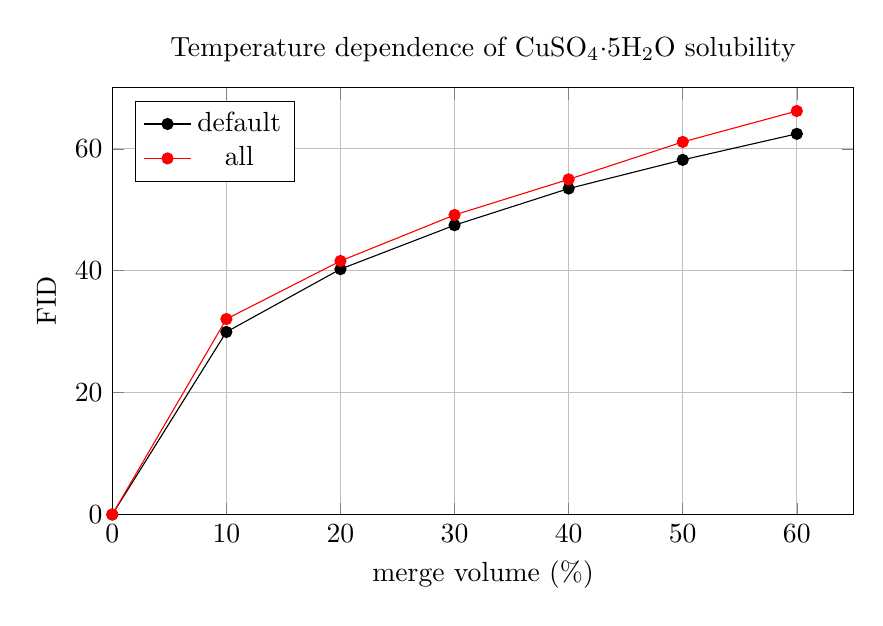
\begin{tikzpicture}
\begin{axis}[
    title={Temperature dependence of CuSO\(_4\cdot\)5H\(_2\)O solubility},
    height=7cm,
    width=11cm,
    xlabel={merge volume (\%)},
    ylabel={FID},
    xmin=0, xmax=65,
    ymin=0, ymax=70,
    xtick={0,10,20,30,40,50,60},
    ytick={0,20,40,60},
    legend pos=north west,
    xmajorgrids=true,
    ymajorgrids=true,
]

\addplot[
    color=black,
    mark=*
    ]
    coordinates {
    (0,0)(10,29.95)(20,40.26)(30,47.47)(40,53.48)(50,58.19)(60,62.46)
    };
    
\addplot[
    color=red,
    mark=*
    ]
    coordinates {
    (0,0)(10,32.07)(20,41.60)(30,49.15)(40,54.99)(50,61.13)(60,66.20)
    };
    
\legend{default, all}
    
\end{axis}
\end{tikzpicture}